\chapter{Weak learners}
\label{chapter:weak learners}

For the reader unfamiliar with tree-based classifiers, this appendix
describes the decision stump and CART algorithms that have been used
in this project.  A much more detailed description is available in
\cite{Cherkassky98}.


\section{Decision stumps}

The decision stump algorithm divides the input space
into two disjoint parts, with the boundary between them running
perpendicular to one of the axes (the decision boundary is an
axis-orthogonal hyperplane).  Each part is given a $y$ value.
Figure \ref{fig:decision stump} shows the two regions of a decision
stump classifier operating on a small, two dimensional, binary
dataset.

\begin{figure}
\begin{center}
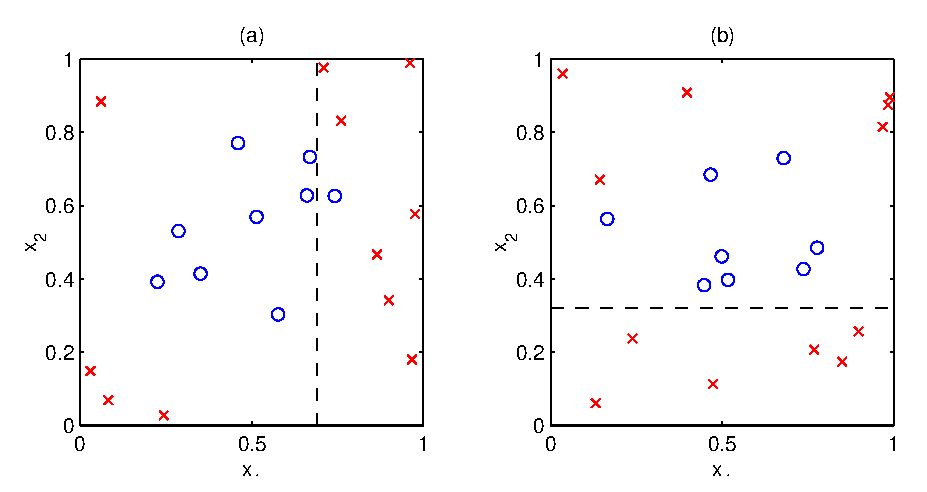
\includegraphics{figures/stumpdiagram.eps}
\end{center}
\caption{Two decision stump classifiers.  Both were trained on the
datasets shown on the plot.  The dotted line represents the decision
boundary.  The label chosen for each region is
simply the label with the highest number of samples within that region.}
\label{fig:decision stump}
\end{figure}

The implementation of the algorithm uses an exhaustive approach to
consider all possible split locations, and chooses the one which
minimises a cost function.  The cost function measures the number of
misclassifications of training samples.

\section{CART}

CART, or ``Classification And Regression Trees'' (see
\cite{Cherkassky98}) is a generalisation of the decision stump
algorithm.  The features of CART are:
%
\begin{itemize}
\item	It is a recursive algorithm, repeatedly subdividing the
	regions until a maximum depth is reached or no subdivision
	improves the performance.  The result is a binary tree.

\item	It is a greedy algorithm, choosing a split which optimises the
	cost function for the particular region it is working on.
	Generally (as with most greedy algorithms) it will not obtain a
	globally optimal classifier.

\item	In order to avoid obtaining a poor classifier, the cost
	function must consider not only the classification error at
	the current depth, but the potential to subdivide in an
	optimal manner also.
\end{itemize}

The original CART algorithm also prunes the tree according to a
separate cost criteria which trades off tree size against
misclassification.  This part of the algorithm has not been
implemented.

Figure \ref{fig:cart} shows the result of running CART on two datasets
drawn from the same distribution.

\begin{figure}
\begin{center}
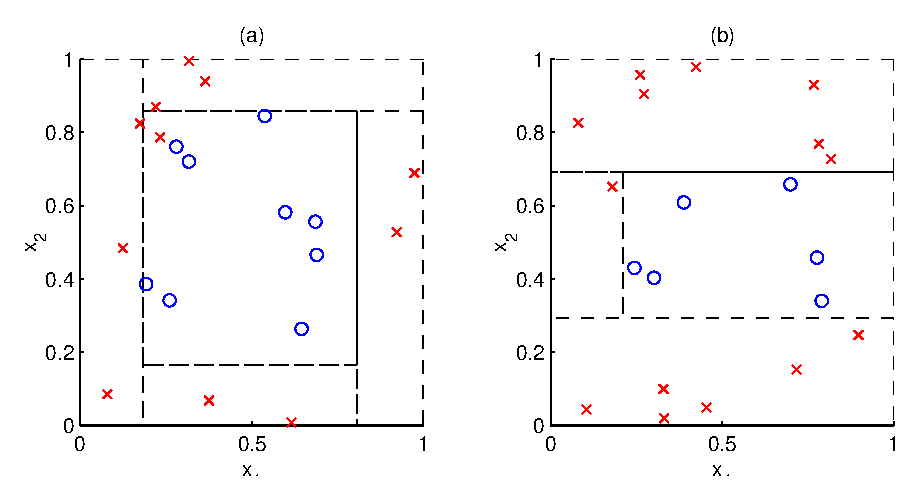
\includegraphics{figures/cartdiagram.eps}
\end{center}
\caption{Two CART classifiers.  Both were trained on the
datasets shown on the plot.  The dotted lines show how the algorithm
breaks the domain into regions.  The label chosen for each region is
simply the label with the highest number of samples within that region.}
\label{fig:cart}
\end{figure}
